\PassOptionsToPackage{unicode=true}{hyperref} % options for packages loaded elsewhere
\PassOptionsToPackage{hyphens}{url}
%
\documentclass[ignorenonframetext,aspectratio=169]{beamer}
\usepackage{pgfpages}
\setbeamertemplate{caption}[numbered]
\setbeamertemplate{caption label separator}{: }
\setbeamercolor{caption name}{fg=normal text.fg}
\beamertemplatenavigationsymbolsempty
% Prevent slide breaks in the middle of a paragraph:
\widowpenalties 1 10000
\raggedbottom
\setbeamertemplate{part page}{
\centering
\begin{beamercolorbox}[sep=16pt,center]{part title}
  \usebeamerfont{part title}\insertpart\par
\end{beamercolorbox}
}
\setbeamertemplate{section page}{
\centering
\begin{beamercolorbox}[sep=12pt,center]{part title}
  \usebeamerfont{section title}\insertsection\par
\end{beamercolorbox}
}
\setbeamertemplate{subsection page}{
\centering
\begin{beamercolorbox}[sep=8pt,center]{part title}
  \usebeamerfont{subsection title}\insertsubsection\par
\end{beamercolorbox}
}
\AtBeginPart{
  \frame{\partpage}
}
\AtBeginSection{
  \ifbibliography
  \else
    \frame{\sectionpage}
  \fi
}
\AtBeginSubsection{
  \frame{\subsectionpage}
}
\usepackage{lmodern}
\usepackage{amssymb,amsmath}
\usepackage{ifxetex,ifluatex}
\usepackage{fixltx2e} % provides \textsubscript
\ifnum 0\ifxetex 1\fi\ifluatex 1\fi=0 % if pdftex
  \usepackage[T1]{fontenc}
  \usepackage[utf8]{inputenc}
  \usepackage{textcomp} % provides euro and other symbols
\else % if luatex or xelatex
  \usepackage{unicode-math}
  \defaultfontfeatures{Ligatures=TeX,Scale=MatchLowercase}
\fi
\usetheme[]{Montpellier}
% use upquote if available, for straight quotes in verbatim environments
\IfFileExists{upquote.sty}{\usepackage{upquote}}{}
% use microtype if available
\IfFileExists{microtype.sty}{%
\usepackage[]{microtype}
\UseMicrotypeSet[protrusion]{basicmath} % disable protrusion for tt fonts
}{}
\IfFileExists{parskip.sty}{%
\usepackage{parskip}
}{% else
\setlength{\parindent}{0pt}
\setlength{\parskip}{6pt plus 2pt minus 1pt}
}
\usepackage{hyperref}
\hypersetup{
            pdftitle={Do Minimum Wages Increase Rents?},
            pdfauthor={Gabriele Borg Diego Gentile Passaro Santiago Hermo},
            pdfborder={0 0 0},
            breaklinks=true}
\urlstyle{same}  % don't use monospace font for urls
\newif\ifbibliography
\setlength{\emergencystretch}{3em}  % prevent overfull lines
\providecommand{\tightlist}{%
  \setlength{\itemsep}{0pt}\setlength{\parskip}{0pt}}
\setcounter{secnumdepth}{0}

% set default figure placement to htbp
\makeatletter
\def\fps@figure{htbp}
\makeatother


\usepackage[backend = biber,
			style = authoryear,
			maxnames = 5,
			maxcitenames = 3,
			doi = false,
			eprint = false]{biblatex}
\addbibresource{../biblio.bib}

\setbeamertemplate{navigation symbols}{}
\setbeamertemplate{footline}[frame number]{}

\AtBeginSubsection{}


\usepackage{multicol}
\newcommand{\btwocol}{\begin{multicols}{2}}
\newcommand{\etwocol}{\end{multicols}}

\usepackage{subcaption}

\newcommand\indep{\protect\mathpalette{\protect\independenT}{\perp}}
\def\independenT#1#2{\mathrel{\rlap{$#1#2$}\mkern2mu{#1#2}}}

\title{Do Minimum Wages Increase Rents?}
\providecommand{\subtitle}[1]{}
\subtitle{Evidence from U.S. Zip Codes Using High Frequency Data}
\author{Gabriele Borg \and Diego Gentile Passaro \and Santiago Hermo}
\date{7/26/2020}

\begin{document}
\frame{\titlepage}

\hypertarget{introduction}{%
\section{Introduction}\label{introduction}}

\begin{frame}{Motivation}
\protect\hypertarget{motivation}{}

Most research on the effects of minimum wage has focused on employment.

--

\end{frame}

\hypertarget{however-as-minimum-wage-policies-are-place-based-it-is-natural-to-expect-broader-effects-in-the-local-economy}{%
\subsection{\texorpdfstring{However, as Minimum wage policies are
\emph{place-based} it is natural to expect broader effects in the local
economy}{However, as Minimum wage policies are place-based it is natural to expect broader effects in the local economy}}\label{however-as-minimum-wage-policies-are-place-based-it-is-natural-to-expect-broader-effects-in-the-local-economy}}

\(\to\) Housing market!

--

A canonical version of the monocentric city model suggests that wage
increases will pass-through to rents.

\begin{frame}{This paper}
\protect\hypertarget{this-paper}{}

In this paper we estimate the effect of minimum wage policies on rents.

\begin{itemize}
\tightlist
\item
  Construct panel dataset at the zipcode-month level using Zillow data
\item
  Show that the panel is representative of the U.S. urban rental market
\item
  Estimate the effect of minimum wage on rents under different
  assumptions
\item
  Propose a novel measure of exposure to minimum wage that exploits the
  place-based nature of the policy.
\item
  Explore heterogeneity of effects based on zipcode characteristics
\end{itemize}

--

We are also working on:

\begin{itemize}
\tightlist
\item
  General equilibrium model of the rental market with a simple labor
  market. This will allow us to be transparent about the mechanisms and
  to do welfare calculations.
\end{itemize}

\end{frame}

\hypertarget{data}{%
\section{Data}\label{data}}

\begin{frame}{Panel dataset}
\protect\hypertarget{panel-dataset}{}

We build a panel at the zipcode-month level from January 2010 to
December 2019:

\begin{itemize}
\tightlist
\item
  Zillow data on rents (median price per square foot of SFCC)
\item
  Minimum wage changes at the state and local levels
\item
  Zipcode characteristics from US Census
\item
  Employment and Average Wages at the county level from QCEW
\item
  Workplace and Residence of workers from LODES
\end{itemize}

\end{frame}

\begin{frame}{Zillow Zip Codes (Map)}
\protect\hypertarget{zillow-zip-codes-map}{}

\begin{figure}
    \caption{Comparison Between Zillow Sample and Population Density}
    \label{fig:maps}
    \begin{subfigure}[b]{\textwidth}\centering
        \includegraphics[width = .85\textwidth]{../../analysis/descriptive_maps/output/sample_map.png}
    \end{subfigure}
    \quad 
    \begin{subfigure}[b]{\textwidth}\centering
        \includegraphics[width = .85\textwidth]{../../analysis/descriptive_maps/output/popurban_density_map.png}
    \end{subfigure}
        \begin{minipage}{.95\textwidth} \footnotesize
        \vspace{2mm} 
        \textit{Notes}: Panel (a) shows the geographical location of the ZIP codes present in the Zillow 
        SFCC sample used in the main analysis. Summary statistics for these units are reported in the main
        paper (\autoref{tab:desc_stats}, column 3). Panel (b) shows the urban population density for the top 
        100 metropolitan areas in the U.S. as reported in the 2008-2011 ACS. Values are winsorized at the 99 
        percentile to provide enough graphical variation.
    \end{minipage}
\end{figure}

\end{frame}

\begin{frame}{Zillow Zip Codes}
\protect\hypertarget{zillow-zip-codes}{}

\begin{table}[h!]
    \caption{Descriptive Statistics of Different Sets of ZIP Codes}
    \centering
    \label{tab:desc_stats}    
    
% Table created by stargazer v.5.2.2 by Marek Hlavac, Harvard University. E-mail: hlavac at fas.harvard.edu
% Date and time: Thu, Nov 05, 2020 - 10:15:39 AM
\begin{tabular}{@{\extracolsep{5pt}} ccccc} 
\\[-1.8ex]\hline 
\hline \\[-1.8ex] 
 & U.S. & Top 100 CBSA & Full Panel & Est. Panel \\ 
\hline \\[-1.8ex] 
Population (millions) (2010) & $311.177$ & $189.712$ & $110.169$ & $50.619$ \\ 
Population as share of U.S. & $1$ & $0.610$ & $0.354$ & $0.163$ \\ 
Housing Units (millions) (2010) & $132.833$ & $78.738$ & $46.722$ & $21.323$ \\ 
Housing Units as share of U.S. & $1$ & $0.593$ & $0.352$ & $0.161$ \\ 
Urban Share (2010) & $0.464$ & $0.754$ & $0.958$ & $0.972$ \\ 
College Share (2010) & $0.464$ & $0.754$ & $0.958$ & $0.972$ \\ 
African-American Share (2010) & $0.464$ & $0.754$ & $0.958$ & $0.972$ \\ 
Hispanic Share (2010) & $0.097$ & $0.136$ & $0.173$ & $0.192$ \\ 
Elder Share (2010) & $0.150$ & $0.130$ & $0.124$ & $0.110$ \\ 
Poor Share (2010) & $0.464$ & $0.754$ & $0.958$ & $0.972$ \\ 
Unemployed Share (2010) & $0.089$ & $0.092$ & $0.092$ & $0.092$ \\ 
Mean HH income (2010) & $52,492.560$ & $62,773.640$ & $65,475.150$ & $66,919.730$ \\ 
Rent House Share (2010) & $0.295$ & $0.347$ & $0.381$ & $0.383$ \\ 
Work in same county share (2010) & $0.701$ & $0.684$ & $0.763$ & $0.756$ \\ 
Unique zipcodes & $38,893$ & $14,583$ & $3,315$ & $1,305$ \\ 
Share of state events & $$ & $$ & $0.030$ & $0.028$ \\ 
Share of county events & $$ & $$ & $0.001$ & $0.001$ \\ 
Share of  localevents & $$ & $$ & $0.003$ & $0.0005$ \\ 
Mean SFCC rent variable & $$ & $$ & $1.304$ & $1.269$ \\ 
Std. Dev. SFCC rent variable & $$ & $$ & $1.033$ & $0.827$ \\ 
Unique zipcodes SFCC rent variable & $$ & $$ & $3,316$ & $1,143$ \\ 
\hline \\[-1.8ex] 
\end{tabular} 

    \begin{minipage}{0.95\textwidth} \footnotesize
        \vspace{3mm} 
        \textit{Notes}: The table shows characteristics of four sets of U.S. postal service 
        ZIP codes. Column 1 reports demographic statistics for the universe of USPS ZIP code 
        we were able to map. Column 2 shows the same statistics for the top 100 Core-Based 
        Statistical Areas (CBSA). Column 3 shows the characteristics of the set of ZIP codes 
        available in the Zillow data. Finally, column 4 shows the restricted balanced sample 
        we use as baseline in our empirical analysis. All demographic information comes from 
        the 2010 Census and the 5-years 2008-2012 ACS.
    \end{minipage}
\end{table}

\end{frame}

\begin{frame}{National Time Series for Zillow and SAFMR data}
\protect\hypertarget{national-time-series-for-zillow-and-safmr-data}{}

\begin{figure}[!h]
    \centering
    \caption{National Time Series for Zillow and SAFMR}
    \label{fig:trend_zillow_safmrwgt}
    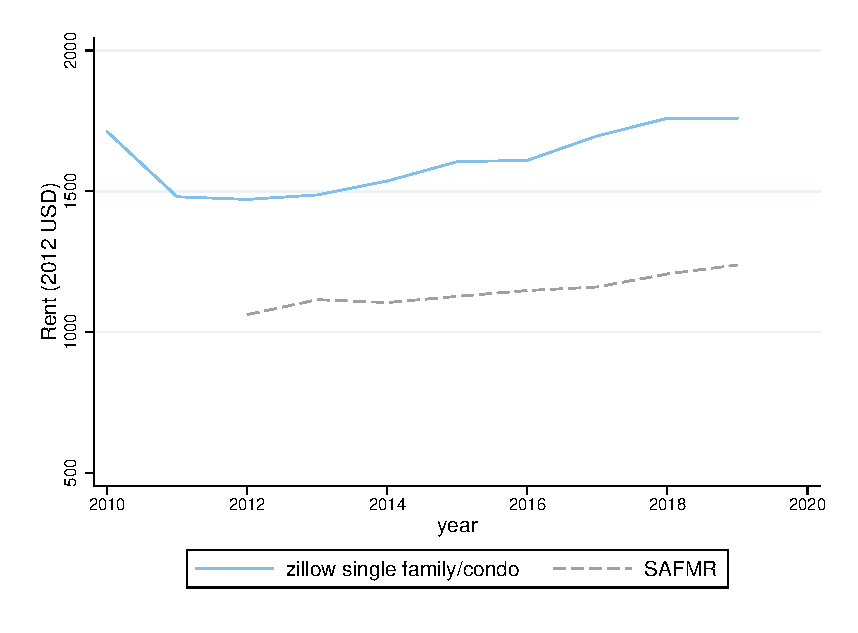
\includegraphics[width = 0.7\textwidth]{../../analysis/zillow_benchmark/output/trend_zillow_safmrwgt_zipcode_avg.eps}
    \begin{minipage}{0.95\textwidth} \footnotesize
        \vspace{3mm}
        \textit{Notes:} The figure plots the annual national average for median rents in the Single 
        Family, Condos and Condominiums category in Zillow, and a weighted combination of SAFMR series 
        with different number of bedrooms. Weights are based on the US share of single family, 
        condos and cooperative houses with given number of bedrooms as recorded in the \textit{American 
        Housing Survey} (\href{https://www.census.gov/programs-surveys/ahs.html}{AHS}). The correlation
        between the series is 0.9406. % See zillow_benchmark make.log
        See footnote \ref{foot:zillow_time_series} in the paper for details on the construction of this 
        time series.  
    \end{minipage}
\end{figure}

\end{frame}

\begin{frame}{Minimum Wage Changes}
\protect\hypertarget{minimum-wage-changes}{}

We use 151 state-level and 182 local-level MW changes, which result in
4224 zipcode-months with changes.

\begin{figure}[h!]
    \centering
    \caption{Distribution of Minimum Wage Changes}
    \label{fig:d_ln_mw_dist}
    \begin{subfigure}{.49\textwidth}
        \caption{Intensity}
        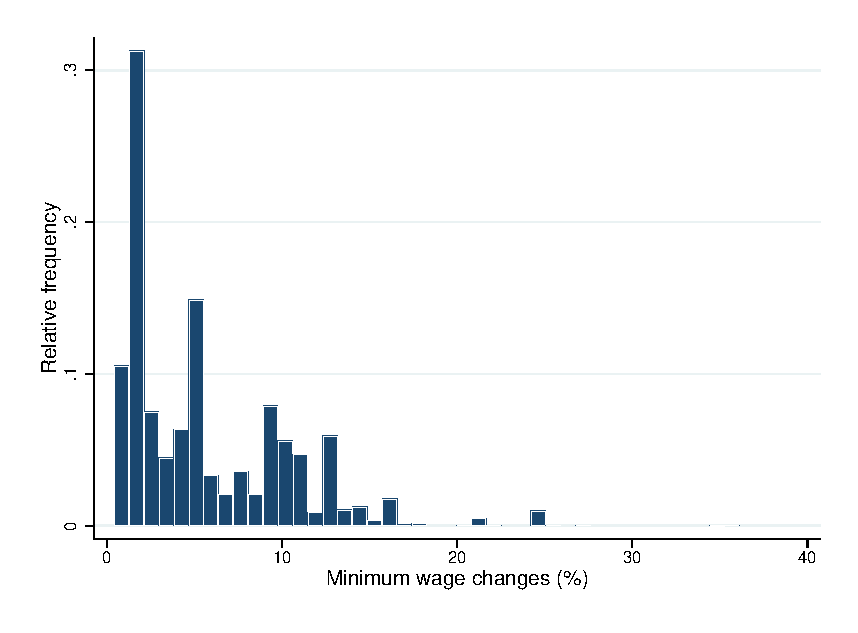
\includegraphics[width = \textwidth]
            {../../analysis/descriptive/output/pct_ch_mw_dist.eps}
    \end{subfigure}
    \begin{subfigure}{.49\textwidth}
        \caption{Timing}
        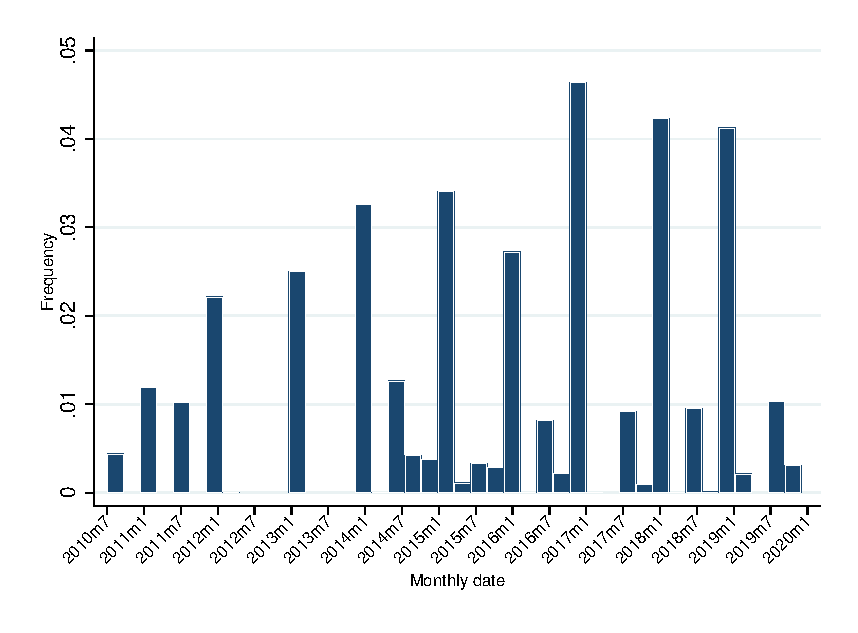
\includegraphics[width = \textwidth]
            {../../analysis/descriptive/output/pct_ch_mw_date_dist.eps}
    \end{subfigure}
    \begin{minipage}{.95\textwidth} \footnotesize
        \vspace{3mm}
        \textit{Notes:} The histograms show the distribution of positive MW changes 
        in the full sample of ZIP codes available in the Zillow data. Panel (a) reports 
        the intensity of the changes in percentage terms. Panel (b) plots the distribution 
        across time of such changes. 
    \end{minipage}
\end{figure}

\end{frame}

\begin{frame}{Using LODES to construct the experienced MW}
\protect\hypertarget{using-lodes-to-construct-the-experienced-mw}{}

Workplace location often differs with residence location. \to Statutory
MW changes are mismeasurement of the actual shift in the wage bill that
determines income at the very local level.

--

Denote ZIP codes by \(i\) and monthly dates by \(t\). Let
\(\mathds{Z}_i\) be the set of ZIP codes in which \(i\)'s residents work
(including \(i\)). We construct the set of weights
\(\{\omega_{iz}\}_{z \in \mathds{Z}_i}\) as
\[\omega_{iz} = \frac{N_{iz}}{N_i} \] where \(N_{iz}\) is the number of
workers who reside in ZIP code \(i\) and work in \(z\), and \(N_i\) is
the total working-age population of ZIP code \(i\). Letting
\(\underline{w}_{it}\) denote the statutory MW in ZIP code \(i\) and
month \(t\), we define the experienced minimum wage measure as:

\begin{equation}
    \underline{w}^{\text{exp}}_{it} = 
            \sum_{z \in \mathds{Z}_i} \omega_{iz} \underline{w}_{zt} \ . 
\end{equation}

\end{frame}

\begin{frame}{Using LODES to construct the experienced MW (Example)}
\protect\hypertarget{using-lodes-to-construct-the-experienced-mw-example}{}

\begin{figure}
    \caption{The California MW Increase of January 2019 in San Diego}
    \label{fig:expmw_san_diego}
    \centering
    \begin{subfigure}[b]{0.65\textwidth}
        \caption{Statutory MW change}
        \includegraphics[width = \textwidth]
            {../../analysis/descriptive_maps/output/San_Diego_mw_msa.png}
    \end{subfigure}\\
    \begin{subfigure}[b]{0.65\textwidth}
        \caption{Experienced MW change}
        \includegraphics[width = \textwidth]
            {../../analysis/descriptive_maps/output/San_Diego_expmw_msa.png}
    \end{subfigure}
    \begin{minipage}{0.95\textwidth} \footnotesize
        \vspace{2mm} 
        \textit{Notes}: The figure maps the percent increase in our minimum wage and 
        experienced minimum wage measures following the state increase in California
        on January 2019. The map colors only those ZIP codes for which we have 
        non-missing rents data from Zillow.
    \end{minipage}
\end{figure}

\end{frame}

\hypertarget{empirical-strategy}{%
\section{Empirical Strategy}\label{empirical-strategy}}

\begin{frame}{Static Difference-in-Differences (DiD) model}
\protect\hypertarget{static-difference-in-differences-did-model}{}

Consider the model \begin{equation}\label{eq:did}
        \Delta y_{it} = \theta_t + \gamma_i + \beta \Delta \underline{w}_{it} + \Delta \epsilon_{it}
\end{equation}

where:

\begin{itemize}
\tightlist
\item
  \(y_{it}\): log rents
\item
  \(\theta_t\) and \(\gamma_i\) are monthly date and zipcode FE
\item
  \(\underline{w}_{it}\) is log actual minimum wage
\item
  \(\epsilon_{it}\) is an error term
\end{itemize}

Identifying assumption: within a zipcode \(\Delta \underline{w}_{it}\)
is mean independent of \(\Delta \epsilon_{it}\) \emph{conditional} on
time fixed effects and a linear trend.

\end{frame}

\begin{frame}{Dynamic models}
\protect\hypertarget{dynamic-models}{}

Consider the model \begin{equation}\label{eq:leads_lags}
    \Delta y_{it} = \theta_t + \gamma_i + \sum_{r=-s}^{s}\beta_r \Delta \underline{w}_{i(t-r)} 
                    + \Delta \epsilon_{it} \ ,
\end{equation} where:

-\(\{\beta_r\}_{r=-s}^{s}\) are dynamic effects of leads and lags of the
minimum wage

\[E \left[ \Delta \epsilon_{it} \Delta \underline{w}_{it-r} \big| \theta_{t}, \gamma_{i} \right] = 0
    \ \ \forall r\in\{-s, ..., -1, 0, 1, ..., s\} \ . \]

Advantages of this specification:

\begin{itemize}
\tightlist
\item
  Test pre-trends assumption
\item
  Assess dynamics of the effect
\end{itemize}

\end{frame}

\hypertarget{results}{%
\subsection{Results}\label{results}}

\begin{frame}{Main Results: DiD}
\protect\hypertarget{main-results-did}{}

\begin{table}[h!]
    \centering
    \resizebox{0.8\textwidth}{!}{
        {
\def\sym#1{\ifmmode^{#1}\else\(^{#1}\)\fi}
\begin{tabular}{l*{3}{c}}
\hline\hline
          &\multicolumn{1}{c}{(1)}&\multicolumn{1}{c}{(2)}&\multicolumn{1}{c}{(3)}\\
          &\multicolumn{1}{c}{D.ln\_med\_rent\_psqft}&\multicolumn{1}{c}{D.ln\_med\_rent\_psqft}&\multicolumn{1}{c}{D.ln\_med\_rent\_psqft}\\
\hline
D.ln\_mw   &   0.0260\sym{**} &   0.0257\sym{**} &   0.0255\sym{**} \\
          & (0.0128)         & (0.0120)         & (0.0117)         \\
\hline
Zipcode-specifc linear trend&       No         &      Yes         &      Yes         \\
Zipcode-specific linear and square trend&       No         &       No         &      Yes         \\
R-squared &    0.022         &    0.024         &    0.026         \\
Observations&   112232         &   112232         &   112232         \\
\hline\hline
\end{tabular}
}
}
    \begin{minipage}{0.9\textwidth} \footnotesize
        \vspace{3mm} 
        \textit{Notes}: The table reports coefficients from versions of the DiD model estimated 
        on the balanced panel of zipcode-months that contains SFCC rental price. Column (1) does 
        corresponds to a two-way fixed effects model estimated in first-differences. Column (2) 
        includes zipcode-specific linear trends, and column (3) allows for zipcode specific quadratic 
        trends. Standard errors clustered at the state level. 
        *** $p < 0.01$, ** $p < 0.05$, * $p < 0.1$.
    \end{minipage}
\end{table}

\end{frame}

\begin{frame}{Main results: Dynamic Models}
\protect\hypertarget{main-results-dynamic-models}{}

\begin{figure}
    \centering
    \includegraphics[width = 0.5\textwidth]{../../analysis/first_differences/output/fd_models.png}
    \begin{minipage}{0.9\textwidth} \footnotesize
        \vspace{2mm} 
        \textit{Notes}: The plot shows the estimated coefficients for alternative models 
        alongside 90 percent confidence intervals. The dashed line additionally reports 
        the point estimate from the DiD. The solid red line show the point 
        estimates for the cumulative effects. Standard errors clustered at the state level.
    \end{minipage}
\end{figure}

\end{frame}

\begin{frame}{Heterogeneity}
\protect\hypertarget{heterogeneity}{}

We interact the DiD model with indicators for quartiles of the
distribution of zipcode characteristics.

\begin{table}[h!]
    \centering
    \resizebox{0.8\textwidth}{!}{
        \vspace{0pt}    
        {
\def\sym#1{\ifmmode^{#1}\else\(^{#1}\)\fi}
\begin{tabular}{l*{4}{c}}
\hline\hline
          &\multicolumn{1}{c}{(1)}&\multicolumn{1}{c}{(2)}&\multicolumn{1}{c}{(3)}&\multicolumn{1}{c}{(4)}\\
          &\multicolumn{1}{c}{Median Income}&\multicolumn{1}{c}{Rental House (\%)}&\multicolumn{1}{c}{College Grad. (\%)}&\multicolumn{1}{c}{African Am. (\%)}\\
\hline
$\Delta \ln(MW) \times 1^{st} qtl$&   0.0395\sym{*}  &   0.0317\sym{*}  &   0.0373\sym{*}  &   0.0178         \\
          & (0.0223)         & (0.0169)         & (0.0196)         & (0.0163)         \\
[1em]
$\Delta \ln(MW) \times 2^{nd} qtl$&   0.0202         &   0.0123         &   0.0473\sym{**} &   0.0218         \\
          & (0.0144)         & (0.0179)         & (0.0222)         & (0.0163)         \\
[1em]
$\Delta \ln(MW) \times 3^{rd} qtl$&   0.0304         &   0.0140         &   0.0258         &   0.0231\sym{*}  \\
          & (0.0252)         & (0.0227)         & (0.0214)         & (0.0133)         \\
[1em]
$\Delta \ln(MW) \times 4^{th} qtl$&   0.0133         &   0.0427\sym{***}&-0.000369         &   0.0419\sym{**} \\
          & (0.0130)         & (0.0156)         & (0.0116)         & (0.0164)         \\
\hline
R-squared &    0.024         &    0.024         &    0.024         &    0.024         \\
Observations&  112,232         &  112,232         &  112,232         &  112,232         \\
\hline\hline
\end{tabular}
}

    }
\end{table}

\end{frame}

\end{document}
